\documentclass[draftclsnofoot,onecolumn,letterpaper,10pt]{IEEEtran}
\pagestyle{empty}
\usepackage{geometry}
\geometry{textheight=9.5in, textwidth=7in}

\usepackage{float}
\usepackage{graphicx}
\newcommand{\subparagraph}{}
\usepackage{titlesec}

\titleformat{\section}[block]{\bfseries\Large}{\thesection}{0.4em}{}
\titleformat{\subsection}[block]{\bfseries\large}{\thesubsection}{0.4em}{}
\titleformat{\subsubsection}[block]{\bfseries\normalsize}{\thesubsubsection}{0.4em}{}
\setlength{\parindent}{0pt}
\renewcommand{\thesection}{\arabic{section}}
\renewcommand{\thesubsection}{\thesection.\arabic{subsection}}
\renewcommand{\thesubsubsection}{\thesubsection.\arabic{subsubsection}}



\date{\today}

\title{brew.ai Design Document}

\begin{document}
{\huge\textbf{Senior Software Engineering Design Group 7}}
	\vspace{1cm}

{\Huge\textbf{brew.ai Design Document}}

\vspace{2cm}
\textbf{Connor Yates} yatesco@oregonstate.edu

\textbf{Aravind Parasurama} parasura@oregonstate.edu

\textbf{Cody Holliday} hollidac@oregonstate.edu

\vspace{2cm}
Sponsor

Dale McCauly, College of Business, Oregon State University

\vspace{0.5cm}
	Approved: \today{}

	Version: 1.0


\newpage
\begin{abstract}
	abstract goes here
\end{abstract}
\newpage
\tableofcontents
\newpage
\section{Introduction}
% Perhaps get rid of these subsection titles, and just combine it into one larger section with appropriate paragraph spacings.
% These talk about the Purpose, scope, etc, of this paper.
\subsection{Purpose}
\subsection{Scope}
\subsection{Context}
\subsection{Summary}

\section{Glossary}

\section{Stakeholders and Design Concerns}
% Here we list out the design concerns of stakeholders (users, etc...) that we address in this document.
% By laying out the design concerns now, we can address each in turn in the subsequent design sections.

\section{Design Viewpoints}
% Details each design point we choose for this project.
% The tech review had 3 technologies, with 3 choices/investigations for each tech.
% Each of the three technologies chosen should be designed in detail in its own "viewpoint".
% each viewpoint then has its own "view". There can be more than one of these.
% the views describe the specific implementations that each viewpoint covers. Refer to the doc for more info.

\subsection{Abstract Learning from Previous Trials} %connor's
From the inception, a major component of this project is the idea that it can learn from mistakes and experiments, and improve the quality of the brew over time.
This section looks at the system design from the viewpoint of artificial intelligence creation.
From this perspective, all other design choices of the project are abstracted into general data sources and sinks.
To further illustrate this point, the view Impact on Other Designs, in Section~\ref{sec:AIImpact}, will introduce the reader to this viewpoint by describing its view of the rest of the system.
From there, the AI system's internal view of the brew.ai system will be explained and designed.

\subsubsection{Impact on Other Designs}\label{sec:AIImpact}
From the viewpoint of learning, the two other major viewpoints, electronic hardware and user interfaces, have little to no impact upon the operations of the system.
There will be interaction between these viewpoints, but that does not imply the other sections will autonomously impact the operation of the system.

From the AI perspective, the system is built as a thinking agent, with the ability to send and receive signals.
This allows the agent to change the world it sees (input signals) through its actions (sent signals).

\begin{figure}
\begin{center}\label{fig:AIsystemDesign}
	\caption{brew.ai System Heirarchy from the viewpoint of the agent}
	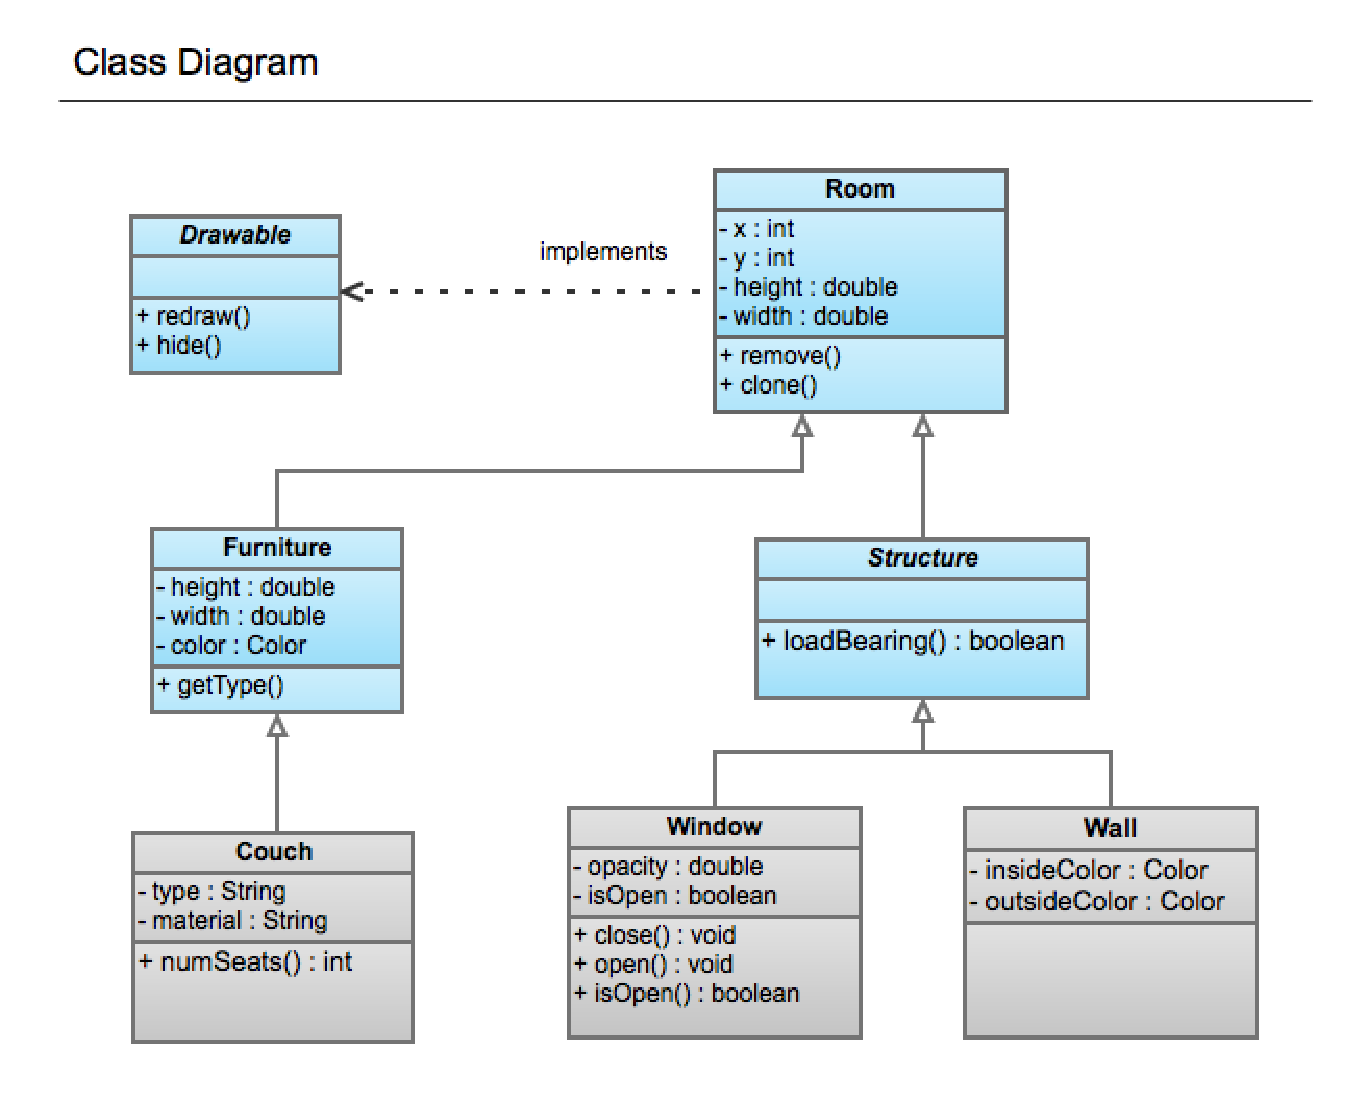
\includegraphics[scale=0.5]{tmp.eps}
\end{center}
\end{figure}
\subsubsection{Learning Algorithm} % Replace with design viewpoint name.
% talk about what algorithm I chose.
% Any design considerations that this algorithm requires
% design of this piece, in the context of the project

\subsubsection{Decision Making Structures}

\subsubsection{Library Implementations}

\subsubsection{Overall Learning Structure}
% diagram showing the interaction between the three previous viewpoints

\subsection{Android-Based User Interface Design} %cody's
\subsubsection{Interface Device}

\subsubsection{UI Connection to controller}

\subsubsection{Dataflow to UI}

\subsubsection{Interface layout}


\subsection{Brewing Hardware and Electronic Controls} %aravind's section

\section{Design Rationale}

\section{Summary}

% References
\bibliography{design_document}
\bibliographystyle{ieeetr}


\end{document}
